% Gallery figure source
% Summary: Crossover recombination creates a chromosome whose left and right parts may have different ancestral histories. Nearby sites are more likely to remain linked.
\documentclass[tikz,border=6pt]{standalone}
% Shared color palette
\usepackage[T1]{fontenc}
\usepackage[utf8]{inputenc}
\usepackage{lmodern}
\usepackage{microtype}
\usepackage{amsmath,amssymb,mathtools}
\usepackage{xcolor}
\usepackage{tikz}
\usetikzlibrary{arrows.meta,positioning,calc,fit,backgrounds,decorations.pathreplacing,shapes.geometric,shadows.blur}

\definecolor{mainblue}{RGB}{42,85,132}
\definecolor{deepgreen}{RGB}{30,105,70}
\definecolor{burntorange}{RGB}{190,90,25}
\definecolor{softgray}{RGB}{245,246,248}
\definecolor{darkgray}{RGB}{70,70,70}
\definecolor{violet}{RGB}{110,70,150}

\newcommand{\given}{\,|\,}
\newcommand{\Ne}{N_{e}}
\newcommand{\ARG}{\mathrm{ARG}}
\newcommand{\MRCA}{\mathrm{MRCA}}
\newcommand{\GMRCA}{\mathrm{GMRCA}}

% Shared TikZ styles
\tikzset{
  tip/.style={circle,fill=black,inner sep=1.6pt},
  nodept/.style={circle,fill=black,inner sep=1.4pt},
  sampled/.style={rectangle,fill=black,inner sep=2.2pt},
  branch/.style={line width=0.8pt},
  retic/.style={circle,draw=burntorange,fill=burntorange!25,line width=0.8pt,inner sep=2.0pt},
  event/.style={circle,draw=mainblue,fill=mainblue!15,line width=0.8pt,inner sep=1.8pt},
  arr/.style={-{Latex[length=2.0mm]},line width=0.8pt},
  faint/.style={line width=0.7pt,draw=gray!55},
  parentedge/.style={-{Latex[length=2.0mm]},line width=0.9pt,draw=burntorange},
  treeedge/.style={-{Latex[length=2.0mm]},line width=0.9pt,draw=black},
  segment/.style={line width=4pt,line cap=round},
  dashedretic/.style={-{Latex[length=2.0mm]},line width=0.9pt,draw=burntorange,dashed}
}


\begin{document}
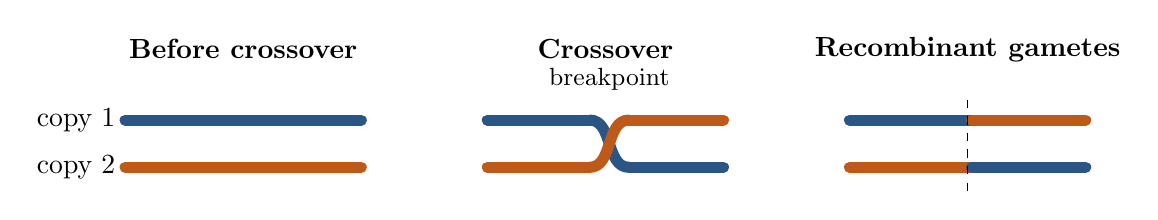
\begin{tikzpicture}[scale=1.0]
  \node[font=\bfseries] at (1.5,2.6) {Before crossover};
  \draw[segment,mainblue] (0,1.7)--(3,1.7);
  \draw[segment,burntorange] (0,1.1)--(3,1.1);
  \node[left] at (0,1.7) {copy 1};
  \node[left] at (0,1.1) {copy 2};

  \begin{scope}[xshift=4.6cm]
  \node[font=\bfseries] at (1.5,2.6) {Crossover};
  \draw[segment,mainblue] (0,1.7)--(1.3,1.7);
  \draw[segment,mainblue] (1.3,1.7).. controls (1.6,1.7) and (1.5,1.1)..(1.8,1.1);
  \draw[segment,mainblue] (1.8,1.1)--(3,1.1);
  \draw[segment,burntorange] (0,1.1)--(1.3,1.1);
  \draw[segment,burntorange] (1.3,1.1).. controls (1.6,1.1) and (1.5,1.7)..(1.8,1.7);
  \draw[segment,burntorange] (1.8,1.7)--(3,1.7);
  \node[above,font=\small] at (1.55,1.95) {breakpoint};
  \end{scope}

  \begin{scope}[xshift=9.2cm]
  \node[font=\bfseries] at (1.5,2.6) {Recombinant gametes};
  \draw[segment,mainblue] (0,1.7)--(1.55,1.7);
  \draw[segment,burntorange] (1.55,1.7)--(3,1.7);
  \draw[segment,burntorange] (0,1.1)--(1.55,1.1);
  \draw[segment,mainblue] (1.55,1.1)--(3,1.1);
  \draw[dashed] (1.5,0.8)--(1.5,2.0);
  \end{scope}
\end{tikzpicture}
\end{document}
